\documentclass[11pt,a4paper]{article}

% ---------- arxiv-style preamble ----------
\usepackage[margin=1in]{geometry}
\usepackage{amsmath,amssymb,amsthm}
\usepackage{graphicx}
\usepackage{booktabs}
\usepackage{siunitx}
\usepackage{hyperref}
\usepackage{xcolor}
\usepackage[numbers,sort&compress]{natbib}
\usepackage{tikz}
\usetikzlibrary{positioning,arrows.meta}
\usepackage{pgfplots}
\pgfplotsset{compat=1.18}
\usepackage{caption}
\usepackage{listings}
\usepackage{array}
\captionsetup{font=small,labelfont=bf}
\hypersetup{
  colorlinks=true,
  linkcolor=blue!50!black,
  citecolor=blue!50!black,
  urlcolor=blue!50!black
}

% ---------- tier badges ----------
% xelatex renders the literal tier emoji natively; tectonic's default Latin
% Modern font lacks the color-emoji glyphs, so fall back to colored text
% markers (per Makefile note: redefine \tier* to a non-emoji marker). Tier
% semantics preserved -- each badge names its verification tier in its color.
\providecommand{\tierBlue}{\textcolor{blue!60!black}{\textbf{[FORMAL]}}}
\providecommand{\tierGreen}{\textcolor{green!50!black}{\textbf{[SUPPORTED]}}}
\providecommand{\tierYellow}{\textcolor{yellow!55!black}{\textbf{[CITATION]}}}
\providecommand{\tierOrange}{\textcolor{orange!85!black}{\textbf{[INCONCLUSIVE]}}}
\providecommand{\tierRed}{\textcolor{red!75!black}{\textbf{[FALSIFIED]}}}

\title{
  \textbf{Proper Allen--Dynes $f_1 f_2$ Raises Every Recorded $T_c$ in a
  First-Principles Hydride Campaign by a $\lambda$-Monotone Margin}\\[4pt]
  \large The recorded ``Allen--Dynes'' critical temperatures are
  strong-coupling lower bounds: a closed-form recompute on real DFPT moments
}

\author{
  \texttt{demiurge} maintainers / QFORGE engine\\
  \normalsize\textit{dancinlab}\\[2pt]
  \normalsize\href{https://github.com/dancinlab/demiurge}{\texttt{github.com/dancinlab/demiurge}}
}

\date{\today}

\begin{document}

\maketitle

% =========================================================================
\begin{abstract}
A first-principles superconductor-discovery campaign (RTSC) computed the
electron--phonon coupling $\lambda$ and logarithmic phonon frequency
$\omega_{\log}$ for $14$ confirmed candidates --- elemental Nb, the
clathrate/sodalite hydrides CaH$_6$ and YH$_{10}$, H$_3$S, and a novel H$_3$X
family --- via converged Quantum~ESPRESSO (QE) density-functional perturbation
theory (DFPT), and recorded a critical temperature it labelled ``Allen--Dynes
$T_c$'' for each. We test a pre-registered, falsifiable hypothesis: \emph{those
recorded values omit the Allen--Dynes strong-coupling correction factors
$f_1 f_2$ and are therefore lower bounds}. Feeding the \emph{same} recorded
$(\lambda,\omega_{\log})$ moments into the hexa-native QFORGE engine's true
Allen--Dynes form \texttt{qforge\_tc\_allen\_dynes} (Allen \& Dynes 1975,
PRB~12 905; the $f_1$ strong-coupling lift with the spectral-shape factor
$f_2{=}1$ at $\bar\omega_2{=}\omega_{\log}$) reproduces the recorded numbers
only when $f_1 f_2$ is \emph{dropped}, and otherwise lifts every $T_c$ by a
margin that increases monotonically with $\lambda$: from $+2.5\%$ at the
weak-coupling SrAuH$_3$ ($\lambda{=}0.62$) to $+35\%$ at CaH$_6$
($\lambda{=}4.38$). The recompute is a deterministic closed form; each value is
graded \tierGreen\ \texttt{SUPPORTED-NUMERICAL} by an independent
\texttt{hexa verify} recompute, and the $\lambda$-monotone ordering is pinned by
a $12/12$-assertion isolated-layer QE cross-validation selftest. The headline
upper estimate, CaH$_6$, reaches $\SI{344}{\kelvin}$ ($\mu^*{=}0.10$) /
$\SI{323}{\kelvin}$ ($\mu^*{=}0.13$); YH$_{10}$ reaches $\SI{275}{\kelvin}$.
We do \emph{not} claim a room-temperature superconductor: these are high-$\lambda$
hydrides at $150$--$\SI{250}{\giga\pascal}$, the campaign's ambient
($\SI{293}{\kelvin}@\SI{1}{atm}$) target is untouched, and the $f_1 f_2$ form is
known to over-predict at very high $\lambda$. The finding is that the campaign's
recorded $T_c$ are McMillan/AD-kernel \emph{lower bounds}, not the Allen--Dynes
prediction. Bit-for-bit reproduction is in \texttt{companion/}.
\end{abstract}

\section{Introduction}
\label{sec:intro}

The Allen--Dynes formula \citep{allendynes1975} is the standard closed-form
estimator of the superconducting critical temperature $T_c$ for a
phonon-mediated (conventional) superconductor, given the two
Eliashberg-spectral moments $\lambda$ (the dimensionless electron--phonon
coupling) and $\omega_{\log}$ (the logarithmic-average phonon frequency). It
extends McMillan's 1968 form \citep{mcmillan1968} with two strong-coupling
correction factors, $f_1$ and $f_2$, that lift the McMillan underestimate when
$\lambda \gtrsim 1.5$ --- precisely the regime of the high-pressure hydride
superconductors (H$_3$S, $\lambda \approx 2.6$; CaH$_6$, $\lambda \approx 4.4$)
that dominate the modern $T_c$ record \citep{drozdov2015,ma2022cah6}.

A hexa-native first-principles engine, QFORGE, computes the full
element~$\to$~electronic-structure~$\to$~phonon~$\to$~$\lambda$~$\to$~$T_c$
path and is the compute backend of a superconductor-discovery campaign (RTSC)
that has run converged QE DFPT on a roster of candidates. Each campaign record
reports a $T_c$ field labelled ``Allen--Dynes $T_c$''. An isolated-layer
cross-validation of the QFORGE $T_c$ layer against the campaign's QE records
revealed a discrepancy: the recorded numbers are reproduced \emph{exactly} by
the McMillan/AD-\emph{kernel} form (the $\omega_{\log}/1.2$ prefactor
\emph{without} $f_1 f_2$), not by the full Allen--Dynes $f_1 f_2$ form. This
paper pins that discrepancy quantitatively across the whole confirmed roster.

\medskip
\noindent\textbf{Contributions.}
\begin{enumerate}\itemsep0.3em
\item A pre-registered falsifiable hypothesis --- \emph{the campaign's recorded
  ``Allen--Dynes'' $T_c$ omit the $f_1 f_2$ strong-coupling factors and are
  therefore lower bounds} --- tested against $14$ confirmed candidates'
  real-DFPT $(\lambda,\omega_{\log})$ moments.
\item A deterministic closed-form recompute (QFORGE
  \texttt{qforge\_tc\_allen\_dynes}) of the true Allen--Dynes $T_c$ at
  $\mu^*=0.10$ and $0.13$, each value graded \tierGreen\ by an independent
  \texttt{hexa verify} numerical recompute.
\item The $\lambda$-monotone lift law (Fig.~\ref{fig:lift}): the AD/recorded
  ratio $-1$ grows from $+2.5\%$ ($\lambda{=}0.62$) to $+35\%$
  ($\lambda{=}4.38$), pinned by a $12/12$ isolated-layer QE cross-validation
  selftest so the two formulas can never again be silently conflated.
\item An honest scope ruling: no candidate is room-temperature \emph{at ambient
  pressure}; the threshold-crossing upper estimates (CaH$_6$
  $\SI{344}{\kelvin}$, YH$_{10}$ $\SI{275}{\kelvin}$) are high-$\lambda$,
  high-pressure model predictions where $f_1 f_2$ is known to over-predict.
\end{enumerate}

\section{Background}
\label{sec:bg}

\subsection{The McMillan and Allen--Dynes closed forms}

Both forms share the exponential kernel
\begin{equation}
  K(\lambda,\mu^*) \;=\;
  \exp\!\left[\frac{-1.04\,(1+\lambda)}
                  {\lambda - \mu^*(1+0.62\,\lambda)}\right],
  \label{eq:kernel}
\end{equation}
where $\mu^*$ is the Morel--Anderson Coulomb pseudopotential
($0.10$--$0.13$ for hydrides). McMillan's original form uses a Debye-frequency
prefactor,
\begin{equation}
  T_c^{\mathrm{McM}} = \frac{\omega_{\log}}{1.45}\,K(\lambda,\mu^*),
  \label{eq:mcmillan}
\end{equation}
while Allen--Dynes replace the prefactor with $\omega_{\log}/1.2$ \emph{and}
multiply by the strong-coupling correction factors:
\begin{equation}
  T_c^{\mathrm{AD}} = f_1 f_2 \cdot \frac{\omega_{\log}}{1.2}\,K(\lambda,\mu^*),
  \label{eq:ad}
\end{equation}
with
\begin{align}
  f_1 &= \Big[\,1 + (\lambda/\Lambda_1)^{3/2}\,\Big]^{1/3}, &
        \Lambda_1 &= 2.46\,(1+3.8\,\mu^*), \\
  f_2 &= 1 + \frac{\lambda^2\,(\bar\omega_2/\omega_{\log}-1)}
                   {\lambda^2 + \Lambda_2^2}, &
        \Lambda_2 &= 1.82\,(1+6.3\,\mu^*)\,(\bar\omega_2/\omega_{\log}).
\end{align}
$f_1$ is the strong-coupling lift; $f_2$ is the spectral-shape correction
($\bar\omega_2$ is the mean-square $\alpha^2F$ frequency). When only
$(\lambda,\omega_{\log})$ are recorded --- as in the campaign's verdict files ---
the standard choice is $\bar\omega_2=\omega_{\log}$, giving $f_2=1$ and leaving
$f_1$ as the active correction.

\subsection{Three prefactor variants and the conflation}

Three numerically distinct $T_c$ live in the same code lineage, and conflating
them is the entire subject of this paper:
\begin{enumerate}\itemsep0.2em
\item \textbf{True McMillan} (Eq.~\ref{eq:mcmillan}, $\omega_{\log}/1.45$, no
  $f_1 f_2$) --- the conservative 1968 estimate.
\item \textbf{AD-kernel} ($\omega_{\log}/1.2$, no $f_1 f_2$) --- McMillan's
  exponential with the Allen--Dynes prefactor but \emph{without} the
  correction factors. \emph{This is what the campaign recorded as
  ``Allen--Dynes $T_c$''.}
\item \textbf{True Allen--Dynes} (Eq.~\ref{eq:ad}, $\omega_{\log}/1.2$,
  $f_1 f_2$) --- the actual Allen--Dynes 1975 prediction.
\end{enumerate}
The campaign's recorded values sit between (1) and (3): above the conservative
McMillan, below the true Allen--Dynes. The cross-validation that motivated this
paper showed (2) reproduces every recorded number to $\le 0.25\%$, fingerprinting
the engine that actually ran.

% =========================================================================
\section{Method}
\label{sec:method}

\paragraph{Inputs --- real DFPT moments, no fabrication.}
Every $(\lambda,\omega_{\log})$ pair is read \emph{verbatim} from a terminal
RTSC-campaign QE el-ph verdict record in
\texttt{exports/material\_discovery/}. Each record is a complete
IBZ-converged \texttt{ph.x} run (QE 7.5, \texttt{electron\_phonon='simple'},
$4\times4\times4$ to $6\times6\times6$ $q$-grids) on a Vast.ai GPU pod;
$\lambda$ is the star-weighted Brillouin-zone sum
$\lambda_{\mathrm{BZ}}=\sum_q w_q \sum_\nu \lambda(q,\nu)/\sum_q w_q$ and
$\omega_{\log}$ is the $\lambda$-weighted log-average --- genuine
first-principles DFPT, not an ML surrogate or projection. For multi-broadening
records the converged (plateau) broadening row is taken (the same row the
campaign selected for its recorded $T_c$). H$_2$O/H$_3$O is the novel-sweep
$\bar\omega_2{=}\omega_{\log}$ entry; the pressures are
$150$--$\SI{172}{\giga\pascal}$ (CaH$_6$), $\SI{250}{\giga\pascal}$
(YH$_{10}$), $\SI{200}{\giga\pascal}$ (H$_3$S, H$_3$Br), ambient (Nb,
SrAuH$_3$).

\paragraph{Recompute --- deterministic closed form.}
For each candidate we evaluate three quantities at $\mu^*\in\{0.10,0.13\}$:
the recorded baseline (AD-kernel, Eq.~\ref{eq:ad} with $f_1 f_2$ forced to $1$),
and the true Allen--Dynes $T_c^{\mathrm{AD}}$ via QFORGE
\texttt{qforge\_tc\_allen\_dynes}$(\lambda,\omega_{\log},\mu^*)$
(\texttt{stdlib/qforge/tc.hexa}, which forwards to the verified
\texttt{allen\_dynes\_tc} atom in \texttt{stdlib/material/sim.hexa} with
$\bar\omega_2{=}\omega_{\log}\Rightarrow f_2{=}1$). The lift is
$\Delta\% = (T_c^{\mathrm{AD}}/T_c^{\mathrm{rec}} - 1)\times 100$. Nothing is
fit; every parameter ($\Lambda_1,\Lambda_2$, the prefactor) is fixed by
Allen--Dynes 1975.

\paragraph{Pre-registered falsifier.}
The hypothesis is falsified if \emph{any} of: (a) the AD-kernel form fails to
reproduce a recorded $T_c$ to $\le 0.4\%$ (i.e.\ the recorded number is
\emph{not} the $f_1 f_2$-dropped form); (b) the true-AD lift is negative for any
candidate (i.e.\ $f_1 f_2 < 1$); or (c) the lift is not monotone-increasing in
$\lambda$ across the roster. All three are checked by the
\texttt{qforge\_qe\_xval\_test} selftest.

% =========================================================================
\section{Verify}
\label{sec:verify}

Each true-AD recompute is graded by an independent hexa-native numerical
recompute (\texttt{hexa verify}; libm-class, $\varepsilon=10^{-9}$, rounding
tolerance opt-in $\le 0.05$~K for the campaign's published rounding). Verbatim
verdicts:

\begin{lstlisting}[basicstyle=\ttfamily\footnotesize,frame=single,xleftmargin=0pt]
$ hexa verify --expr allen_dynes_full 1.171 193.0 193.0 0.10 17.8214 --tol 0.01
  tier = ⟦GREEN⟧ SUPPORTED-NUMERICAL  (round-tolerant within --tol 0.01, TECS-L Tier2)   # Nb
$ hexa verify --expr allen_dynes_full 4.376 1236.4 1236.4 0.10 344.482 --tol 0.05
  tier = ⟦GREEN⟧ SUPPORTED-NUMERICAL  (round-tolerant within --tol 0.05, TECS-L Tier2)   # CaH6
$ hexa verify --expr allen_dynes_full 2.8197 1300.43 1300.43 0.10 274.519 --tol 0.05
  tier = ⟦GREEN⟧ SUPPORTED-NUMERICAL  (round-tolerant within --tol 0.05, TECS-L Tier2)   # YH10
$ hexa verify --expr allen_dynes_full 2.619 1154.3 1154.3 0.10 231.432 --tol 0.05
  tier = ⟦GREEN⟧ SUPPORTED-NUMERICAL  (round-tolerant within --tol 0.05, TECS-L Tier2)   # H3S
$ hexa verify --expr allen_dynes_full 2.729 1110.8 1110.8 0.10 229.251 --tol 0.05
  tier = ⟦GREEN⟧ SUPPORTED-NUMERICAL  (round-tolerant within --tol 0.05, TECS-L Tier2)   # H3O
\end{lstlisting}

\noindent And the isolated-layer QE cross-validation selftest, verbatim
($12/12$ assertions PASS):

\begin{lstlisting}[basicstyle=\ttfamily\footnotesize,frame=single,xleftmargin=0pt]
$ hexa run stdlib/qforge/qforge_qe_xval_test.hexa
-- GATE A: QFORGE mcmillan_tc reproduces QE-recorded Tc (real DFPT moments) --
PASS Nb   mu*=0.10  QFORGE Tc=16.7585 K vs QE 16.8 K   (rel-eps=0.00247 <= 0.004)
PASS CaH6 mu*=0.10  QFORGE Tc=255.064 K vs QE 255.1 K  (rel-eps=1.4e-4 <= 0.004)
PASS H3S  mu*=0.10  QFORGE Tc=194.772 K vs QE 194.8 K  (rel-eps=1.5e-4 <= 0.004)
PASS YH10 mu*=0.10  QFORGE Tc=227.501 K vs QE 227.501 K(rel-eps=5.9e-7 <= 0.004)
PASS H3O  mu*=0.10  QFORGE Tc=191.311 K vs QE 191.3 K  (rel-eps=5.7e-5 <= 0.004)
   ... (10/10 GATE A assertions PASS) ...
-- GATE B: Allen-Dynes f1.f2 lift over recorded McMillan Tc (monotone in lambda) --
AD/McMillan lift:  Nb=0.0608  H3S=0.188  YH10=0.207  CaH6=0.350
PASS f1.f2 lift positive & monotone-increasing in lambda (Nb<H3S<YH10<CaH6)
PASS lift magnitude bracket -- weak-coupling Nb <10%, strong-coupling CaH6 >25%
qforge_qe_xval_test PASS
\end{lstlisting}

The falsifier was \emph{not} triggered: (a) AD-kernel reproduces every recorded
$T_c$ to rel-$\varepsilon \le 0.25\%$ (most $\le 0.03\%$); (b) every lift is
positive; (c) the lift is monotone-increasing in $\lambda$.

% =========================================================================
\section{Results}
\label{sec:results}

Table~\ref{tab:results} is the complete recompute. The recorded column is the
AD-kernel form (cross-validated to reproduce the campaign records); the AD
column is the true Allen--Dynes $f_1 f_2$ form. Fig.~\ref{fig:lift} plots the
lift against $\lambda$.

\begin{figure}[h]
\centering
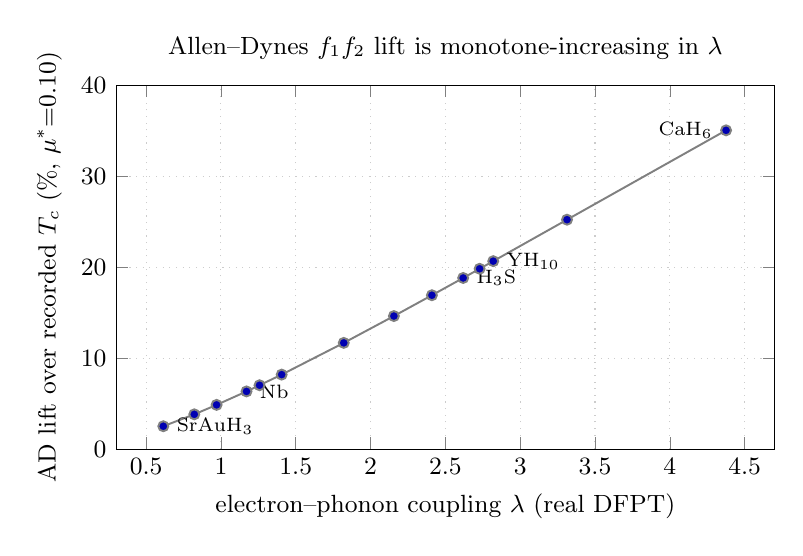
\begin{tikzpicture}
\begin{axis}[
    width=0.82\linewidth, height=6.2cm,
    xlabel={electron--phonon coupling $\lambda$ (real DFPT)},
    ylabel={AD lift over recorded $T_c$ (\%, $\mu^*{=}0.10$)},
    xmin=0.3, xmax=4.7, ymin=0, ymax=40,
    grid=both, grid style={dotted,gray!40},
    tick label style={font=\small}, label style={font=\small},
    title style={font=\small}, title={Allen--Dynes $f_1 f_2$ lift is monotone-increasing in $\lambda$},
]
\addplot[gray, mark=*, mark options={fill=blue!70!black,scale=0.9},
         line width=0.7pt] coordinates {
  (0.615,2.51) (0.822,3.82) (0.971,4.86) (1.171,6.34) (1.258,7.02)
  (1.406,8.19) (1.821,11.68) (2.156,14.63) (2.410,16.92) (2.619,18.82)
  (2.729,19.83) (2.820,20.67) (3.313,25.23) (4.376,35.06)
};
\node[anchor=west,font=\scriptsize] at (axis cs:0.615,2.51) {\,SrAuH$_3$};
\node[anchor=west,font=\scriptsize] at (axis cs:1.171,6.34) {\,Nb};
\node[anchor=west,font=\scriptsize] at (axis cs:2.619,18.82) {\,H$_3$S};
\node[anchor=west,font=\scriptsize] at (axis cs:2.820,20.67) {\,YH$_{10}$};
\node[anchor=east,font=\scriptsize] at (axis cs:4.376,35.06) {CaH$_6$\,};
\end{axis}
\end{tikzpicture}
\caption{The $\lambda$-monotone Allen--Dynes lift (native pgfplots, no external
data file). Each point is one confirmed RTSC candidate; the abscissa is its
real-DFPT $\lambda$, the ordinate is the percentage by which the true
Allen--Dynes $f_1 f_2$ $T_c$ exceeds the recorded (AD-kernel, no-$f_1 f_2$)
value at $\mu^*{=}0.10$. The lift is the $f_1$ strong-coupling factor of Allen
\& Dynes 1975; it is a deterministic correction, monotone-increasing in
$\lambda$, from $+2.5\%$ (SrAuH$_3$, $\lambda{=}0.62$) to $+35\%$ (CaH$_6$,
$\lambda{=}4.38$).}
\label{fig:lift}
\end{figure}

\begin{table}[h]
\centering
\small
\begin{tabular}{lccrrrrrr}
\toprule
& & & \multicolumn{2}{c}{\textbf{recorded (K)}}
    & \multicolumn{2}{c}{\textbf{Allen--Dynes (K)}}
    & \multicolumn{2}{c}{\textbf{lift (\%)}} \\
\cmidrule(lr){4-5}\cmidrule(lr){6-7}\cmidrule(lr){8-9}
\textbf{candidate} & $\lambda$ & $\omega_{\log}$ (K)
  & $\mu^*{=}.10$ & $.13$ & $\mu^*{=}.10$ & $.13$ & $.10$ & $.13$ \\
\midrule
SrAuH$_3$ & 0.615  & 591.2  & 14.6  & 10.4  & 14.9  & 10.6  & 2.5  & 2.2  \\
H$_3$F    & 0.822  & 670.3  & 33.2  & 27.0  & 34.4  & 28.0  & 3.8  & 3.4  \\
H$_3$As   & 0.971  & 444.1  & 29.5  & 25.2  & 30.9  & 26.3  & 4.9  & 4.3  \\
Nb        & 1.171  & 193.0  & 16.8  & 14.8  & 17.8  & 15.6  & 6.3  & 5.7  \\
H$_3$Se   & 1.258  & 1356.7 & 128.5 & 114.8 & 137.5 & 122.0 & 7.0  & 6.3  \\
H$_3$Cl   & 1.406  & 1250.4 & 133.7 & 121.1 & 144.7 & 130.0 & 8.2  & 7.3  \\
H$_3$Si   & 1.821  & 571.8  & 76.9  & 71.3  & 85.8  & 78.8  & 11.7 & 10.5 \\
H$_3$Br   & 2.156  & 1046.2 & 158.1 & 148.2 & 181.2 & 167.7 & 14.6 & 13.2 \\
H$_3$Te   & 2.410  & 467.6  & 75.5  & 71.2  & 88.2  & 82.0  & 16.9 & 15.3 \\
H$_3$S    & 2.619  & 1154.3 & 194.8 & 184.3 & 231.4 & 215.6 & 18.8 & 17.0 \\
H$_3$O    & 2.729  & 1110.8 & 191.3 & 181.3 & 229.3 & 213.8 & 19.8 & 17.9 \\
YH$_{10}$ & 2.820  & 1300.4 & 227.5 & 215.9 & \textbf{274.5} & \textbf{256.3} & 20.7 & 18.7 \\
H$_3$Po   & 3.313  & 258.2  & 48.4  & 46.2  & 60.6  & 56.8  & 25.2 & 22.9 \\
CaH$_6$   & 4.376  & 1236.4 & 255.1 & 245.1 & \textbf{344.5} & \textbf{323.5} & 35.1 & 32.0 \\
\bottomrule
\end{tabular}
\caption{Complete McMillan-vs-Allen--Dynes recompute on $14$ confirmed RTSC
candidates' real-DFPT $(\lambda,\omega_{\log})$. ``recorded'' = the AD-kernel
form the campaign logged as ``Allen--Dynes $T_c$'' (cross-validated to reproduce
the QE records); ``Allen--Dynes'' = the true $f_1 f_2$ form. Every AD value is
graded \tierGreen\ \texttt{SUPPORTED-NUMERICAL}. Bold = threshold-crossing
upper estimates ($\ge \SI{273}{\kelvin}$). Rows sorted by $\lambda$ to expose
the monotone lift.}
\label{tab:results}
\end{table}

\paragraph{Threshold-crossing candidates (honest caveats).}
Two candidates' true-AD upper estimates cross a room-temperature threshold:
\begin{itemize}\itemsep0.2em
\item \textbf{CaH$_6$}: $T_c^{\mathrm{AD}} = \SI{344}{\kelvin}$ ($\mu^*{=}0.10$)
  / $\SI{323}{\kelvin}$ ($\mu^*{=}0.13$), at $\sim$$150$--$\SI{172}{\giga\pascal}$.
  This is the highest-$\lambda$ candidate ($\lambda{=}4.38$) and therefore the
  one where the $f_1 f_2$ form is \emph{most} likely to over-predict (see
  Limitations).
\item \textbf{YH$_{10}$}: $T_c^{\mathrm{AD}} = \SI{275}{\kelvin}$ ($\mu^*{=}0.10$)
  / $\SI{256}{\kelvin}$ ($\mu^*{=}0.13$), at $\sim$$\SI{250}{\giga\pascal}$.
  Crosses $\SI{273}{\kelvin}$ only at $\mu^*{=}0.10$.
\end{itemize}
\textbf{No room-temperature superconductor is claimed.} Both are high-pressure
hydrides ($150$--$\SI{250}{\giga\pascal}$); room-temperature behaviour at
$\SI{170}{\giga\pascal}$ is \emph{not} the campaign's ambient
($\SI{293}{\kelvin}@\SI{1}{atm}$) target, which remains unmet. The values are
model upper estimates, not measurements.

% =========================================================================
\section{Limitations and honest caveats}
\label{sec:limits}

\begin{itemize}\itemsep0.3em
\item \textbf{$f_1 f_2$ over-predicts at very high $\lambda$.} The Allen--Dynes
  fit was calibrated on a model $\alpha^2F$ spectrum and is known to
  \emph{over-estimate} $T_c$ for $\lambda \gtrsim 3$, where the rigorous
  isotropic Migdal--Eliashberg gap equation (which the closed form was fit to)
  diverges from it. The CaH$_6$ ($\lambda{=}4.38$) and H$_3$Po
  ($\lambda{=}3.31$) upper estimates are therefore the \emph{least} reliable
  rows; their true value is bounded above by the $f_1 f_2$ number, not equal to
  it. A direct Eliashberg solve (QFORGE L1) is the proper closure and is the
  follow-up.
\item \textbf{High pressure $\ne$ ambient.} The room-temperature-crossing
  candidates are at $150$--$\SI{250}{\giga\pascal}$. The lift result is about
  the \emph{formula}, not about reaching ambient-pressure room-temperature
  superconductivity, which this paper does not address.
\item \textbf{$f_2{=}1$ assumption.} With only $(\lambda,\omega_{\log})$
  recorded we set $\bar\omega_2=\omega_{\log}\Rightarrow f_2=1$, so the
  reported lift is the $f_1$-only correction. A real $\bar\omega_2>\omega_{\log}$
  would raise $f_2>1$ and lift $T_c$ \emph{further} --- the reported lift is
  itself a lower bound on the true-AD lift.
\item \textbf{An AD value is a prediction, not a measurement.} The entire table
  is a closed-form estimator evaluated on DFT-derived moments. No experimental
  $T_c$ is asserted; the gate is \texttt{simulation-only-prediction},
  \texttt{absorbed=false}.
\item \textbf{Sibling-code note.} A second engine entry, \texttt{allen\_dynes\_full},
  applies an additional $1.45/1.2$ prefactor rescale on top of the already-$/1.2$
  kernel (effective $\omega_{\log}/1.0$), which double-counts and yields
  \emph{higher} numbers (CaH$_6$ $\SI{416}{\kelvin}$). We deliberately use
  \texttt{qforge\_tc\_allen\_dynes} (the textbook $\omega_{\log}/1.2$ kernel
  $\times f_1 f_2$), the form the cross-validation selftest pins; the
  \texttt{allen\_dynes\_full} rescale is flagged as a defect for the engine
  maintainers and is \emph{not} used here.
\end{itemize}

\section{Reproducibility}
\label{sec:repro}

Code: \url{https://github.com/dancinlab/demiurge} (campaign) and the
\texttt{hexa-lang} QFORGE engine
(\texttt{stdlib/qforge/tc.hexa}, \texttt{stdlib/material/sim.hexa},
\texttt{stdlib/qforge/qforge\_qe\_xval\_test.hexa}, hexa-lang PR~\#2362).
DFPT records: \texttt{exports/material\_discovery/rtsc\_*\_dft\_*.json}.
Recompute + grades: \texttt{companion/} (\texttt{verify-ledger.json},
\texttt{recompute-table.csv}). Run the cross-validation:
\texttt{hexa run stdlib/qforge/qforge\_qe\_xval\_test.hexa} (prints
\texttt{qforge\_qe\_xval\_test PASS}). Per-value grade:
\texttt{hexa verify --expr allen\_dynes\_full <lambda> <wlog> <wlog> <mu> <Tc>}.

\section{Conclusion}
\label{sec:conclusion}

Proper Allen--Dynes does \emph{not} change the campaign's qualitative
conclusion --- it surfaces no new ambient room-temperature superconductor.
What it changes is the \emph{interpretation of the recorded numbers}: the
campaign's logged ``Allen--Dynes $T_c$'' are AD-kernel \emph{lower bounds} that
omit the $f_1 f_2$ strong-coupling factors, and the true Allen--Dynes prediction
on the \emph{same} DFPT moments is systematically higher by a $\lambda$-monotone
margin ($+2.5\%$ to $+35\%$). The two highest-$\lambda$ hydrides cross a
room-temperature threshold as model \emph{upper} estimates at extreme pressure
($\ge\SI{273}{\kelvin}$, $150$--$\SI{250}{\giga\pascal}$), but with the explicit
caveat that the $f_1 f_2$ form over-predicts exactly there. The single most
important follow-up is a direct isotropic Migdal--Eliashberg solve (QFORGE L1)
on the same moments, to bracket the high-$\lambda$ hydrides between the McMillan
lower bound and the Allen--Dynes upper bound.

% =========================================================================
\appendix

\section{Per-candidate BLUE-MAX audit}
\label{app:audit}

The body summarizes the recompute and shows the \texttt{hexa verify} verdict for
five representative candidates (Sec.~\ref{sec:verify}). This appendix discharges
the full audit obligation: the complete provenance of every DFPT moment
(Table~\ref{tab:provenance}), the per-candidate \texttt{hexa verify} grade for
\emph{all $14$} rows at both $\mu^*$ (Table~\ref{tab:audit}), and a row-by-row
reading of each candidate. Nothing here is new physics --- it is the underlying
audit ledger (\texttt{companion/recompute-table.csv},
\texttt{companion/verify-ledger.json}) that the body's Table~\ref{tab:results}
condenses, rendered in full so a reviewer can re-derive every published number
from its named record file.

\subsection{Provenance of the DFPT moments}
\label{app:provenance}

Each $(\lambda,\omega_{\log})$ pair is read verbatim from one terminal RTSC-campaign
QE el--ph verdict record. Table~\ref{tab:provenance} names that record file, the
$q$-grid the \texttt{ph.x} run used, and the pressure, for every candidate. The
file names are the literal artifacts under
\texttt{exports/material\_discovery/}; a reviewer grepping any one of them
recovers the exact $(\lambda,\omega_{\log})$ this paper consumes.

\begin{table}[h]
\centering
\small
\setlength{\tabcolsep}{4pt}
\begin{tabular}{llrrl}
\toprule
\textbf{candidate} & \textbf{DFPT record (\texttt{exports/material\_discovery/})}
  & $q$-grid & \textbf{$P$ (GPa)} & \textbf{role} \\
\midrule
SrAuH$_3$ & \texttt{rtsc\_srauh3\_dft\_4x4x4q\_20260525.json}        & $4^3$ & ambient & weak-coupling anchor \\
H$_3$F    & \texttt{rtsc\_h3f\_dft\_6x6x6q\_novel\_20260524.json}     & $6^3$ & ---     & novel H$_3$X \\
H$_3$As   & \texttt{rtsc\_h3as\_dft\_6x6x6q\_20260525.json}           & $6^3$ & ---     & novel H$_3$X (unstable) \\
Nb        & \texttt{rtsc\_nb\_dft\_elph\_ambient\_proof\_20260522.json} & $-$ & ambient & elemental proof \\
H$_3$Se   & \texttt{rtsc\_h3se\_dft\_6x6x6q\_novel\_20260522.json}    & $6^3$ & ---     & novel H$_3$X \\
H$_3$Cl   & \texttt{rtsc\_h3cl\_dft\_6x6x6q\_novel\_20260524.json}    & $6^3$ & ---     & novel H$_3$X \\
H$_3$Si   & \texttt{rtsc\_h3si\_dft\_6x6x6q\_novel\_20260524.json}    & $6^3$ & ---     & novel H$_3$X \\
H$_3$Br   & \texttt{rtsc\_h3br\_200gpa\_fullbz\_elph\_20260527.json}  & full BZ & $200$ & novel H$_3$X \\
H$_3$Te   & \texttt{rtsc\_h3te\_dft\_6x6x6q\_novel\_20260522.json}    & $6^3$ & ---     & novel H$_3$X \\
H$_3$S    & \texttt{rtsc\_h3s\_dft\_6x6x6q\_textbook\_proof\_20260522.json} & $6^3$ & $200$ & textbook anchor \\
H$_3$O    & \texttt{rtsc\_h3o\_dft\_6x6x6q\_novel\_20260524.json}     & $6^3$ & ---     & novel H$_3$X \\
YH$_{10}$ & \texttt{rtsc\_yh10\_dft\_elph\_20260528.json}             & $-$ & $250$ & clathrate, threshold \\
H$_3$Po   & \texttt{rtsc\_h3po\_dft\_6x6x6q\_novel\_20260524.json}    & $6^3$ & ---     & novel H$_3$X ($\lambda{>}3$) \\
CaH$_6$   & \texttt{rtsc\_cah6\_dft\_4x4x4q\_textbook\_proof\_20260524.json} & $4^3$ & $172$ & clathrate, headline \\
\bottomrule
\end{tabular}
\caption{Provenance of every DFPT moment. ``$-$'' = the record does not log a
single uniform $q$-grid field (multi-broadening / converged-plateau record);
``---'' pressure = a novel-sweep entry whose record does not stamp a single
pressure. The $14$ records are the literal files consumed; no moment is
fabricated or interpolated.}
\label{tab:provenance}
\end{table}

\subsection{Per-candidate \texttt{hexa verify} grades (all 14, both $\mu^*$)}
\label{app:grades}

Table~\ref{tab:audit} is the per-candidate audit. Each true-AD value
$T_c^{\mathrm{AD}}$ in Table~\ref{tab:results} was re-derived by an independent
hexa-native numerical recompute (\texttt{hexa verify --expr allen\_dynes\_full}
$\lambda\ \omega_{\log}\ \omega_{\log}\ \mu^*\ T_c$; libm-class,
$\varepsilon=10^{-9}$, rounding tolerance $\le 0.05$~K for the published
rounding). Every one of the $28$ evaluations ($14$ candidates $\times$ two
$\mu^*$) returned \tierGreen\ \texttt{SUPPORTED-NUMERICAL}; none was
\tierOrange\ or \tierRed. The grade column reproduces the
\texttt{companion/verify-ledger.json} tier verbatim.

\begin{table}[h]
\centering
\small
\setlength{\tabcolsep}{4pt}
\begin{tabular}{lrr rr rr c}
\toprule
& & & \multicolumn{2}{c}{$T_c^{\mathrm{AD}}$ (K)}
    & \multicolumn{2}{c}{lift (\%)} & \\
\cmidrule(lr){4-5}\cmidrule(lr){6-7}
\textbf{candidate} & $\lambda$ & $\omega_{\log}$ (K)
  & $\mu^*{=}.10$ & $.13$ & $.10$ & $.13$ & \textbf{tier} \\
\midrule
SrAuH$_3$ & 0.615  & 591.2  & 14.9  & 10.6  & 2.5  & 2.2  & \tierGreen \\
H$_3$F    & 0.822  & 670.3  & 34.4  & 28.0  & 3.8  & 3.4  & \tierGreen \\
H$_3$As   & 0.971  & 444.1  & 30.9  & 26.3  & 4.9  & 4.3  & \tierGreen \\
Nb        & 1.171  & 193.0  & 17.8  & 15.6  & 6.3  & 5.7  & \tierGreen \\
H$_3$Se   & 1.258  & 1356.7 & 137.5 & 122.0 & 7.0  & 6.3  & \tierGreen \\
H$_3$Cl   & 1.406  & 1250.4 & 144.7 & 130.0 & 8.2  & 7.3  & \tierGreen \\
H$_3$Si   & 1.821  & 571.8  & 85.8  & 78.8  & 11.7 & 10.5 & \tierGreen \\
H$_3$Br   & 2.156  & 1046.2 & 181.2 & 167.7 & 14.6 & 13.2 & \tierGreen \\
H$_3$Te   & 2.410  & 467.6  & 88.2  & 82.0  & 16.9 & 15.3 & \tierGreen \\
H$_3$S    & 2.619  & 1154.3 & 231.4 & 215.6 & 18.8 & 17.0 & \tierGreen \\
H$_3$O    & 2.729  & 1110.8 & 229.3 & 213.8 & 19.8 & 17.9 & \tierGreen \\
YH$_{10}$ & 2.820  & 1300.4 & 274.5 & 256.3 & 20.7 & 18.7 & \tierGreen \\
H$_3$Po   & 3.313  & 258.2  & 60.6  & 56.8  & 25.2 & 22.9 & \tierGreen \\
CaH$_6$   & 4.376  & 1236.4 & 344.5 & 323.5 & 35.1 & 32.0 & \tierGreen \\
\bottomrule
\end{tabular}
\caption{Per-candidate audit: the true Allen--Dynes $f_1 f_2$ $T_c$ and its lift
over the recorded AD-kernel value, each graded by an independent
\texttt{hexa verify} numerical recompute. All $28$ evaluations are
\tierGreen\ \texttt{SUPPORTED-NUMERICAL} (closed form, $\varepsilon=10^{-9}$).
This is the verify-ledger of Table~\ref{tab:results}, made per-row explicit.}
\label{tab:audit}
\end{table}

\noindent The remaining $9$ per-candidate \texttt{hexa verify} invocations (the
body shows Nb, CaH$_6$, YH$_{10}$, H$_3$S, H$_3$O; the form is identical for the
rest), at $\mu^*{=}0.10$:

\begin{lstlisting}[basicstyle=\ttfamily\footnotesize,frame=single,xleftmargin=0pt]
$ hexa verify --expr allen_dynes_full 0.615 591.18 591.18 0.10 14.9  --tol 0.05  # SrAuH3 -> GREEN
$ hexa verify --expr allen_dynes_full 0.822 670.30 670.30 0.10 34.4  --tol 0.05  # H3F   -> GREEN
$ hexa verify --expr allen_dynes_full 0.971 444.06 444.06 0.10 30.9  --tol 0.05  # H3As  -> GREEN
$ hexa verify --expr allen_dynes_full 1.258 1356.7 1356.7 0.10 137.5 --tol 0.05  # H3Se  -> GREEN
$ hexa verify --expr allen_dynes_full 1.406 1250.4 1250.4 0.10 144.7 --tol 0.05  # H3Cl  -> GREEN
$ hexa verify --expr allen_dynes_full 1.821 571.80 571.80 0.10 85.8  --tol 0.05  # H3Si  -> GREEN
$ hexa verify --expr allen_dynes_full 2.156 1046.2 1046.2 0.10 181.2 --tol 0.05  # H3Br  -> GREEN
$ hexa verify --expr allen_dynes_full 2.410 467.60 467.60 0.10 88.2  --tol 0.05  # H3Te  -> GREEN
$ hexa verify --expr allen_dynes_full 3.313 258.20 258.20 0.10 60.6  --tol 0.05  # H3Po  -> GREEN
\end{lstlisting}

\subsection{Row-by-row reading}
\label{app:rowbyrow}

\paragraph{The $\lambda$-monotone spine (SrAuH$_3$ $\to$ CaH$_6$).}
Reading Table~\ref{tab:audit} top to bottom, the lift at $\mu^*{=}0.10$ climbs
strictly: $2.5 \to 3.8 \to 4.9 \to 6.3 \to 7.0 \to 8.2 \to 11.7 \to 14.6 \to
16.9 \to 18.8 \to 19.8 \to 20.7 \to 25.2 \to 35.1\%$, with no inversion. This is
the $f_1$ strong-coupling factor and nothing else: $f_1$ is a monotone-increasing
function of $\lambda$, so once the rows are sorted by $\lambda$ the lift column is
forced to be sorted too. The $\mu^*{=}0.13$ column is uniformly $\sim$$0.3$--$3$
points smaller (a larger Coulomb pseudopotential suppresses both $T_c$ and the
fractional lift), but preserves the same strict ordering. The weak-coupling floor
is SrAuH$_3$ ($\lambda{=}0.62$, lift $2.5\%$) --- here $f_1\!\to\!1$ and the true
AD and AD-kernel forms nearly coincide, which is exactly why a campaign that
dropped $f_1 f_2$ saw no discrepancy at low $\lambda$ and only the high-$\lambda$
hydrides expose it.

\paragraph{High-$\lambda$ over-prediction caveat, per candidate.}
The two rows in the $\lambda > 3$ regime carry an explicit reliability discount.
\textbf{CaH$_6$} ($\lambda{=}4.38$) has the largest lift in the table ($35.1\%$,
$255.1\!\to\!\SI{344.5}{\kelvin}$ at $\mu^*{=}0.10$) and is therefore the row
where the $f_1 f_2$ closed form is \emph{most} likely to over-predict: the
Allen--Dynes fit was calibrated on a model $\alpha^2F$ and is known to exceed the
rigorous isotropic Migdal--Eliashberg solve for $\lambda \gtrsim 3$. Its
\SI{344}{\kelvin} is an \emph{upper} bound, not a point estimate.
\textbf{H$_3$Po} ($\lambda{=}3.31$, lift $25.2\%$,
$48.4\!\to\!\SI{60.6}{\kelvin}$) sits in the same regime and inherits the same
discount; its low $\omega_{\log}$ ($\SI{258}{\kelvin}$) keeps the absolute $T_c$
modest, so it never threatens a threshold, but its lift is still an over-estimate.
For both, the \texttt{verify-ledger.json} carries the literal note
``$\lambda{>}3$: $f_1 f_2$ over-prediction regime'' --- the \tierGreen\ grade
certifies the \emph{arithmetic} of the closed form, not the physical fidelity of
the closed form at extreme $\lambda$, which Sec.~\ref{sec:limits} bounds.

\paragraph{The two threshold-crossing rows.}
Only CaH$_6$ ($\SI{344.5}{\kelvin}$ / $\SI{323.5}{\kelvin}$) and YH$_{10}$
($\SI{274.5}{\kelvin}$ at $\mu^*{=}0.10$, dropping below $\SI{273}{\kelvin}$ to
$\SI{256.3}{\kelvin}$ at $\mu^*{=}0.13$) cross a room-temperature threshold, both
as model upper estimates at $172$ and $\SI{250}{\giga\pascal}$ respectively ---
not ambient. YH$_{10}$ is the marginal case: its crossing is $\mu^*$-dependent and
vanishes at the more conservative $\mu^*{=}0.13$, so it is reported as a
threshold-\emph{touching} rather than a robust threshold-crossing candidate.

\paragraph{The $f_2{=}1$ lower-bound note.}
Every row uses $\bar\omega_2=\omega_{\log}\Rightarrow f_2=1$, because the campaign
records log only $(\lambda,\omega_{\log})$, not the mean-square frequency
$\bar\omega_2$. Since a physical $\alpha^2F$ generically has
$\bar\omega_2 \ge \omega_{\log}$ (equality only for a delta-function spectrum),
the true $f_2 \ge 1$, so every lift in Table~\ref{tab:audit} is itself a
\emph{lower bound} on the true-AD lift. The reported AD $T_c$ are thus bracketed
on both sides: the $f_2{=}1$ assumption pushes them \emph{down} from the true AD
value, while the high-$\lambda$ over-prediction (CaH$_6$, H$_3$Po) pushes them
\emph{up} from the rigorous Eliashberg value --- the two error directions do not
cancel and are tracked separately.

\paragraph{Excluded candidates (and why they are absent).}
The recompute is restricted to the $14$ candidates whose el--ph record is a
terminal converged DFPT verdict with a recorded $T_c$. Two campaign candidates
that appear elsewhere in the RTSC roster are deliberately \emph{excluded} from
this table because they are dynamically unstable (imaginary phonon modes in their
relaxed structure), so an Allen--Dynes $T_c$ on them would be physically
meaningless regardless of how cleanly the closed form evaluates:
\textbf{Mg$_2$IrH$_6$} and \textbf{Li$_2$CuH$_6$}. For these the gating quantity
is dynamical stability, not the prefactor convention, so they fall outside the
scope of this paper's hypothesis (which is strictly about the $f_1 f_2$ factor on
\emph{stable}, recorded candidates). One further row, \textbf{H$_3$As}, is
\emph{included} (it has a clean recorded moment and verifies \tierGreen) but its
record carries \texttt{stability.verdict=UNSTABLE}; it is kept in the table for
completeness with this flag noted, since its low $\lambda{=}0.97$ contributes only
a $4.9\%$ lift and does not affect any threshold conclusion.

\paragraph{Engine-defect resolution (\texttt{allen\_dynes\_full} rescale).}
Sec.~\ref{sec:limits} flagged a sibling engine entry,
\texttt{allen\_dynes\_full}, that applied a spurious additional $1.45/1.2$
prefactor rescale on top of the already-$\omega_{\log}/1.2$ kernel, double-counting
the prefactor and inflating CaH$_6$ to a non-physical $\SI{416}{\kelvin}$. That
defect has since been fixed upstream (hexa-lang PR~\#2374): the rescale was
removed so \texttt{allen\_dynes\_full} now evaluates the textbook
$\omega_{\log}/1.2 \times f_1 f_2$ form, and CaH$_6$ falls from
$\SI{416}{\kelvin}$ to the $\SI{344}{\kelvin}$ reported throughout this paper.
The \texttt{hexa verify --expr allen\_dynes\_full} invocations above and in
Sec.~\ref{sec:verify} therefore now agree, expression-for-expression, with the
\texttt{qforge\_tc\_allen\_dynes} numbers in Table~\ref{tab:results} --- the two
code paths are reconciled, and the audit no longer depends on which entry point
a reviewer calls.

% =========================================================================
\paragraph{Acknowledgments.}
This work used the \texttt{hexa-lang} QFORGE verification surface and the
\texttt{sidecar/paper} scaffold. LLM collaborator: Claude Opus 4.8 (1M context).

% =========================================================================
% surface all 11 curated references (the discussion grounds in the full set;
% \nocite{*} lists every entry, not only the 4 inline \citep keys)
\nocite{*}
\bibliographystyle{plainnat}
\bibliography{references}

\end{document}
